
\noindent Recall the generating function for a single-variable Gaussian probability distribution $e^{\frac{1}{2} a x^2}$ and the moment-generating integral

\begin{equation}
I = \int_{-\infty}^\infty dx \,\, x^{2n} e^{\frac{1}{2} a x^2} = \frac{(2n-1)!!}{a^n}.
\end{equation}

\noindent We also derived the identity with the generating function for the multivariable Gaussian probability distribution

\begin{equation}
\int_{-\infty}^\infty dx_1 \dots \int_{-\infty}^\infty dx_n \,\, e^{-\frac{1}{2} x^T \textbf{A} x + J^T x} = \sqrt{\frac{\pi^n}{\text{det}(\textbf{A})}} e^{J^T \textbf{A}^{-1} J}.
\end{equation}

\noindent The 2-point correlation function for the $n$-variable Gaussian is (\textbf{Exercise}), for $j \ne k$

\begin{equation}
\langle x_j x_k \rangle \equiv \frac{\int_{-\infty}^\infty dx_1 \dots \int_{-\infty}^\infty dx_n \,\, x_j x_k e^{-\frac{1}{2} x^T \textbf{A} x}}{\int_{-\infty}^\infty dx_1 \dots \int_{-\infty}^\infty dx_n \,\, e^{-\frac{1}{2} x^T \textbf{A} x}} \equiv[\textbf{A}^{-1}]_{jk}.
\end{equation}

\noindent Note that this is also equal to the second derivative with respect to the vector $J$, evaluated at $J=0$

\begin{equation}
\langle x_j x_k \rangle \equiv \frac{\frac{\partial^2}{\partial J_j \partial J_k}\int_{-\infty}^\infty dx_1 \dots \int_{-\infty}^\infty dx_n \,\, e^{-\frac{1}{2} x^T \textbf{A} x + J^T x} }{\int_{-\infty}^\infty dx_1 \dots \int_{-\infty}^\infty dx_n \,\, e^{-\frac{1}{2} x^T \textbf{A} x + J^T x}} \Big|_{J=0}.
\end{equation}

\subsection*{Higher Order Moments: $l$-point Correlation Functions}

\noindent The $l$-point correlation function has similar form

\begin{equation}
\langle x_{j_1} \dots x_{j_l} \rangle \equiv \frac{\int_{-\infty}^\infty dx_{j_1} \dots \int_{-\infty}^\infty dx_{j_l} \,\, x_{j_1} \dots x_{j_l} \,\, e^{-\frac{1}{2} x^T \textbf{A} x}}{\int_{-\infty}^\infty dx_{j_1} \dots \int_{-\infty}^\infty dx_{j_l} \,\, e^{-\frac{1}{2} x^T \textbf{A} x}}.
\end{equation}

\noindent By Wick's theorem (proof by induction), for even $l$, the $l$-point correlation function is proportional to the sum of the products over the permutation group on $l$ symbols, the "Wick sum". We write "proportional to" for reasons of symmetry and soon eliminating redundant terms.

\begin{equation}
\langle x_{j_1} \dots x_{j_l} \rangle \propto \sum_{\pi \in S_l} [\textbf{A}^{-1}]_{ j_{\pi^{-1}(1)}j_{\pi^{-1}(2)}} \dots [\textbf{A}^{-1}]_{j_{\pi^{-1}(l-1)}j_{\pi^{-1}(l)}} .
\end{equation}

\subsubsection*{Example: 4-point Correlation}

\noindent To calculate the 4-point correlation function, we begin by considering the $4!=24$ total permutations on 4 symbols. Since $\textbf{A}^{-1}$ is symmetric

\begin{equation}
[\textbf{A}^{-1}]_{jk} = [\textbf{A}^{-1}]_{kj} 
\end{equation}

\noindent And there are only $\frac{24}{2! 2! 2!} = 3$ unique terms (products of two matrix elements), which are (\textbf{Exercise})

\begin{align*}
\langle x_{j_1} x_{j_2} x_{j_3} x_{j_4} \rangle &= [\textbf{A}^{-1}]_{j_1 j_2} [\textbf{A}^{-1}]_{j_3 j_4} \\
&+ [\textbf{A}^{-1}]_{j_1 j_3} [\textbf{A}^{-1}]_{j_2 j_4} \\
&+ [\textbf{A}^{-1}]_{j_1 j_4} [\textbf{A}^{-1}]_{j_2 j_3} \\
&= \langle x_{j_1} x_{j_2} \rangle \langle x_{j_3} x_{j_4} \rangle + \langle x_{j_1} x_{j_3} \rangle \langle x_{j_2} x_{j_4} \rangle + \langle x_{j_1} x_{j_4} \rangle \langle x_{j_2} x_{j_3} \rangle
\end{align*}

\noindent With the approporiate choice of $\textbf{A}$, in the context of path integrals and perturbative field theory, these products of correlations functions are exactly correspondent to Feynman propagator, and, in turn, the Feynman diagrams, just as we studied in \textit{Lecture 9} of the last lecture series (Quantum Field Theory) for the 4-particle Wick contraction.

\begin{figure}[H]
	\centering
	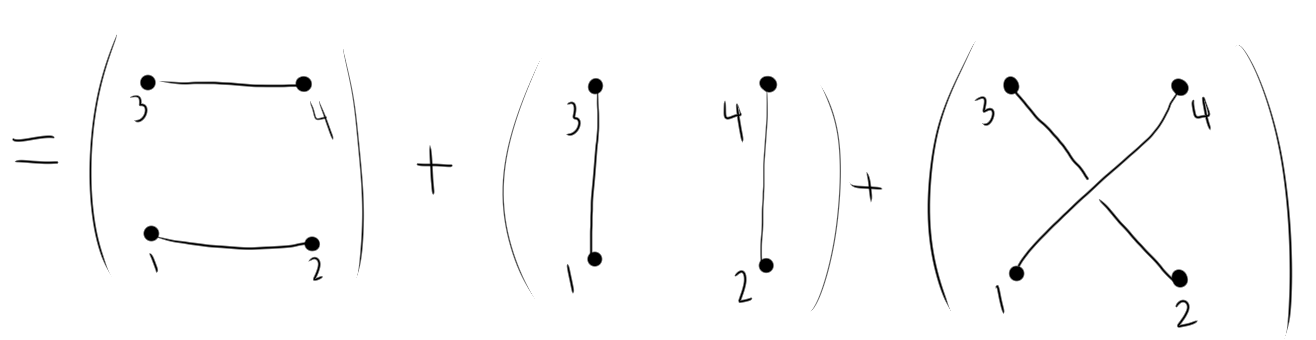
\includegraphics[scale=0.5]{images/feynman4point.png}
	\caption{Feynman diagram correspondence  of the 4-point correlation function}
\end{figure}

\noindent Keeping only unique terms, the proprotionality relation becomes an equivalence

\begin{equation}
\langle x_{j_1} \dots x_{j_l} \rangle  = \sum_{\text{unique} \,\pi^{-1}} [\textbf{A}^{-1}]_{ j_{\pi^{-1}(1)}j_{\pi^{-1}(2)}} \dots [\textbf{A}^{-1}]_{j_{\pi^{-1}(l-1)}j_{\pi^{-1}(l)}} 
\end{equation}

\noindent (\textbf{Exercise}) Calculate the 6-point correlation function with $\frac{6!}{2! 2! 2!} = 90$ unique terms

\begin{equation}
\langle x_{j_1} x_{j_2} x_{j_3} x_{j_4} x_{j_5} x_{j_6} \rangle = [\textbf{A}^{-1}]_{j_1 j_2} [\textbf{A}^{-1}]_{j_3 j_4}  [\textbf{A}^{-1}]_{j_5 j_6} + \dots
\end{equation}

\noindent In short summary,

\begin{itemize}
\item We can calculate \textit{all} moments for the Gaussian probability distribution.
\item We have a diagrammatic calculus to calculate the $l$-point correlation functions, which end up being exactly the Feynman propagators/diagrams, with appropriate choice of $\textbf{A}$, and is the direct connection of quantum field theory and Gaussian integrals.
\end{itemize}

\subsection*{The Matrix \textbf{A} for Path Integrals}

\noindent Let the potential $V$ be quadratic in the canonical position coordinate per particle $q_k$ (e.g., a one-dimensional chain of oscillators), such that the transition amplitude, which will be discretized, evaluated, and limited $\epsilon \rightarrow 0$, from some state $q_a$ to another $q_b$ is

\begin{equation}
U(q_a, q_b; T) = \left( \prod_k \int \frac{dq_k}{c(\epsilon)} \right) e^{\frac{1}{2} i q^T \textbf{A} q}
\end{equation}

\noindent Where we know the quadratic form contains a kinetic energy term plus a potential energy term

\begin{equation}
q^T \textbf{A} q = \sum_k \left( m \frac{(q_{k+1} - q_k}{\epsilon}^2 - \epsilon V (\frac{q_{k+1} + q_k}{2}) \right).
\end{equation}

\noindent This results is $\textbf{A}$ as a \textit{tridiagonal} matrix for the kinetic energy term and a potential energy term which is a matrix with elements quadratic in $q$

\begin{equation}
\textbf{A} = 
\begin{bmatrix}
    \frac{2m}{\epsilon} & -\frac{m}{\epsilon} & 0 & \cdots & & & \\
    -\frac{m}{\epsilon} & \frac{2m}{\epsilon} & -\frac{m}{\epsilon} & 0 & \cdots & & \\
    0 & -\frac{m}{\epsilon} & \frac{2m}{\epsilon}& -\frac{m}{\epsilon}& 0 & \cdots \\
    \vdots & 0 &\ddots & \ddots & \ddots
\end{bmatrix}
+ [V( q^2 )]
\end{equation}

\noindent The transition amplitude is then calculated similarly to last lecture as

\begin{equation}
U(q_a, q_b; T) = \frac{ \infty \, \text{const.}}{\sqrt{\text{det}(\textbf{A})}}
\end{equation}

\noindent The infinite constant will not be a problem since the $l$-point correlation is normalized, and the same exact infinite constant will appear in the denominator and cancel the constant. So, in terms of $q_k$, the $l$-point correlation reads

\begin{equation}
\langle q_{j_1} \dots q_{j_l} \rangle \equiv \frac{\prod_k \int \frac{dq_k}{c(\epsilon)} q_{j_1} \dots q_{j_l} \,\, e^{-\frac{1}{2} i q^T \textbf{A} x}}{\prod_k \int \frac{dq_k}{c(\epsilon)} \,\, e^{-\frac{1}{2} i q^T \textbf{A} x}}.
\end{equation}

\noindent Note that with periodic boundary conditions, the elements of follow a modulo relation $\textbf{A}_{jk} = f((j-k) \, \text{mod} \, n)$, where $n$ is the number of sites/oscillators in the chain. \\

\noindent Assuming that $\textbf{A}$ is invertible, there exists a unitary matrix $Q$, such that $Q^T Q = \mathbb{I}$ and $Q^T \textbf{A} Q = D$, with diagonal matrix $D$ with the eigenvalues of $\textbf{A}$ along the diagonal. Then the determinant of $\textbf{A}$ is easy to calculate, since 

\begin{equation}
\text{det}(\textbf{A}) = \prod_{j=1}^n \lambda_j (\textbf{A}).
\end{equation}

\subsection*{Correlations Functions and Quantum Observables}

\noindent Consider the transition amplitude over 2-point spatial correlations

\begin{equation}
U(q_a, q_b; T) \propto \int \mathcal{D} \phi(x) \,\, \phi(x_1) \phi(x_2) e^{i \int_{-T}^T d^4 x \, \mathcal{L}(\phi)}
\end{equation}

\noindent With an expression like this, always discretize by sending $\phi(x_j) \rightarrow q_j$, evaluate the integral, and enter the contiuum limit with the boundary conditions

\begin{align}
\phi (-T, x) &= \phi_a (x) \\
\phi (T, x) &= \phi_b (x).
\end{align}

\noindent Apply the following condition, exploiting the boundary conditions, to factor the full field "integral" over the individual fields and the boundary of the field

\begin{equation}
\int \mathcal{D} \phi (x) = \int \mathcal{D} \phi_1 (x) \int \mathcal{D} \phi_2 (x) \int_{\partial \phi} \mathcal{D} \phi (x)
\end{equation}

\noindent Where the boundary $\partial \phi = \partial \phi_1 + \partial \phi_2$ is defined by 

\begin{align}
\phi_1 (x) = \phi(x_1^0, x_1) \\
\phi_2 (x) = \phi(x_2^0, x_2)
\end{align}

\noindent So, after performing the boundary integral, we introduce quantum stuff to the expression from the classical 2-point function above, for $x_2^0 > x_1^0$

\begin{align*}
U(q_a, q_b; T) \propto \int \mathcal{D} \phi_1 (x) \int \mathcal{D} \phi_2 (x) \,\, &\phi(x_1) \phi(x_2) \bra{\phi_b} e^{-i \hat{H} (T-x_2^0)} \ket{\phi_2} \\
 &\times \bra{\phi_2} e^{-i \hat{H} (x_2^0 - x_1^0)} \ket{\phi_1} \bra{\phi_1} e^{-i \hat{H} (x_1^0 + T)} \ket{\phi_a}
\end{align*}

\noindent Now, apply the Schroedinger-picture field operator to write the classical field operators in terms of quantum field operators. The formula is

\begin{equation}
\hat{\phi}_S (x) \ket{\phi_1} = \phi (x_1) \ket{\phi_1}
\end{equation}

\noindent So, the purely quantum expression for the 2-point function is

\begin{align*}
U(q_a, q_b; T) \propto\int \mathcal{D} \phi_1 (x) \int \mathcal{D} \phi_2 (x) \,\, &\bra{\phi_b} e^{-i \hat{H} (T-x_2^0)} \hat{\phi}_S (x) \ket{\phi_2} \\
 &\times \bra{\phi_2} e^{-i \hat{H} (x_2^0 - x_1^0)} \hat{\phi}_S (x) \ket{\phi_1} \bra{\phi_1} e^{-i \hat{H} (x_1^0 + T)} \ket{\phi_a}
\end{align*}

\noindent This is called the time-ordered expectation value of the field operators in the Heisenberg picture. The equation holds for $x_2^0 < x_1^0$ as well, and we can write it as

\begin{equation}
U(q_a, q_b; T) \propto \bra{\phi_b} e^{-i \hat{H} T} \mathcal{T}[ \hat{\phi}_H (x_1) \hat{\phi}_H (x_2)] e^{-i \hat{H} T} \ket{\phi_a}
\end{equation}

\noindent Now, enter the limit as $T \rightarrow \infty$, where we bring the interacting vacuum state and the normalization for the full transition amplitude (\textbf{Exercise}), and introduce the \textit{most important formula} for this course

\begin{equation}
\bra{\Omega} \mathcal{T} [ \hat{\phi}_H (x_1) \hat{\phi}_H (x_2) ] \ket{\Omega} = \lim_{T \rightarrow \infty (1-i\epsilon)} \frac{\int \mathcal{D} \phi \,\, \phi (x_1) \phi (x_2) e^{i \int_{-T}^T d^4 x \, \mathcal{L} (\phi)}}{\int \mathcal{D} \phi \,\, e^{i \int_{-T}^T d^4 x \, \mathcal{L} (\phi)}}.
\end{equation}

\noindent So, the LHS is built of purely quantum observables equal to the classical expression of path integrals! \\

\noindent This expression will end up to be the propagator, which is also the inverse of the Klein-Gordon operator, which is what we call $\textbf{A}$ in the scalar quantum field theory. \\

\noindent The solution to this is well-known for the case when $\mathcal{L}$ is quadratic in the field operators, and one can easily discretize, evaluate the Gaussian integral, and take the limit as $\epsilon \rightarrow 0$. \\

\noindent \textbf{(Exercise)} Calculate the $l$-point formula for the time-ordered expectation value of the field operators in the Heisenberg picture.